\section{Señales AM}
Se estudiaron señales moduladas en AM generadas con dos osciloscopios, de forma que la frecuencia de la portadora sea de $1MHz$ con amplitud de $250 mV_{pp}$ y la frecuencia de la moduladora de $100 KHz$

Sea $S_{AM}(t)$ la señal modulada, $S_p(t)$ la señal portadora y $S_M(t)$ la señal moduladora, entonces 
\begin{equation}
    S_p(t)=A_pcos(2\pi f_pt)
\label{eq:Sp}
\end{equation}

\begin{equation}
    S_M=\frac{1}{2}mA_pcos(2\pi f_Mt)
\label{eq:Sm}
\end{equation}
siendo $A_p$ la amplitud de la señal portadora, $m$ el coeficiente de modulación, definido según $m=\frac{V_{max}-V_{min}}{V_{max}+V_{min}}$, y $f_p$ y $f_M$ la frecuencia de la señal portadora y la señal moduladora respectivamente.

La señal modulada puede describirse como la suma de tres señales senoidales de tres frecuencias distintas, una central y otras dos que la modulan. Matemáticamente es posible describirla según la siguiente ecuación:

\begin{equation}
    S_{AM}(t)=S_p(t)(1+mS_M(t))
    \label{eq:sam2}
\end{equation}

Desarrollando,
\begin{equation}
    S_{AM}=\frac{1}{2}A_pcos(2\pi f_pt)+\frac{1}{2}mA_p(cos(2\pi (f_p-f_M)t)+cos(2\pi (f_p+f_M)t))
    \label{eq:Sam}
\end{equation}

\subsection{Señal senoidal AM m=0,5}

Para el primer caso se moduló una señal AM con $m=0,5$. El espectro observado se presenta en las figuras \ref{fig:am01} y \ref{fig:am02}

\begin{figure}[H]
  \centering
  \begin{minipage}[b]{0.6\textwidth}
    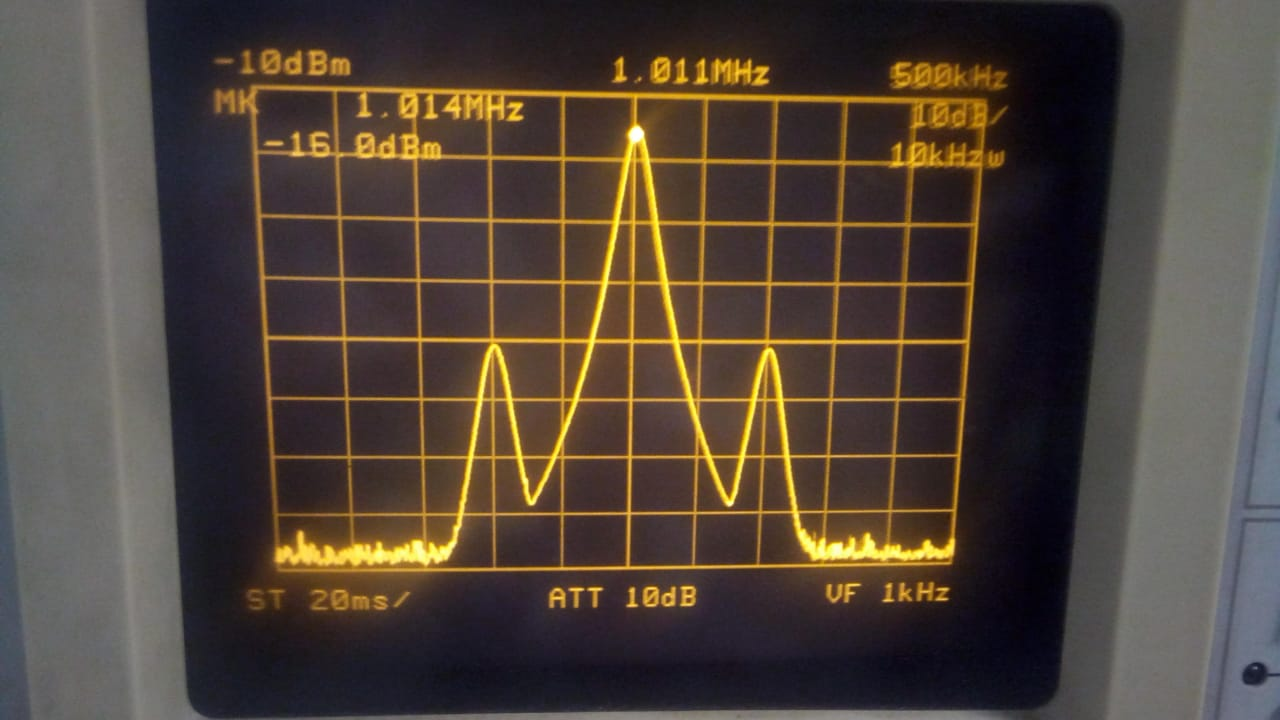
\includegraphics[width=\textwidth]{/ImagenesEjercicio3y4/AM05_3.jpeg}
    \caption{Espectro de la señal AM con m=0,5}
    \label{fig:am01}
  \end{minipage}
  \hfill
  \begin{minipage}[b]{0.6\textwidth}
    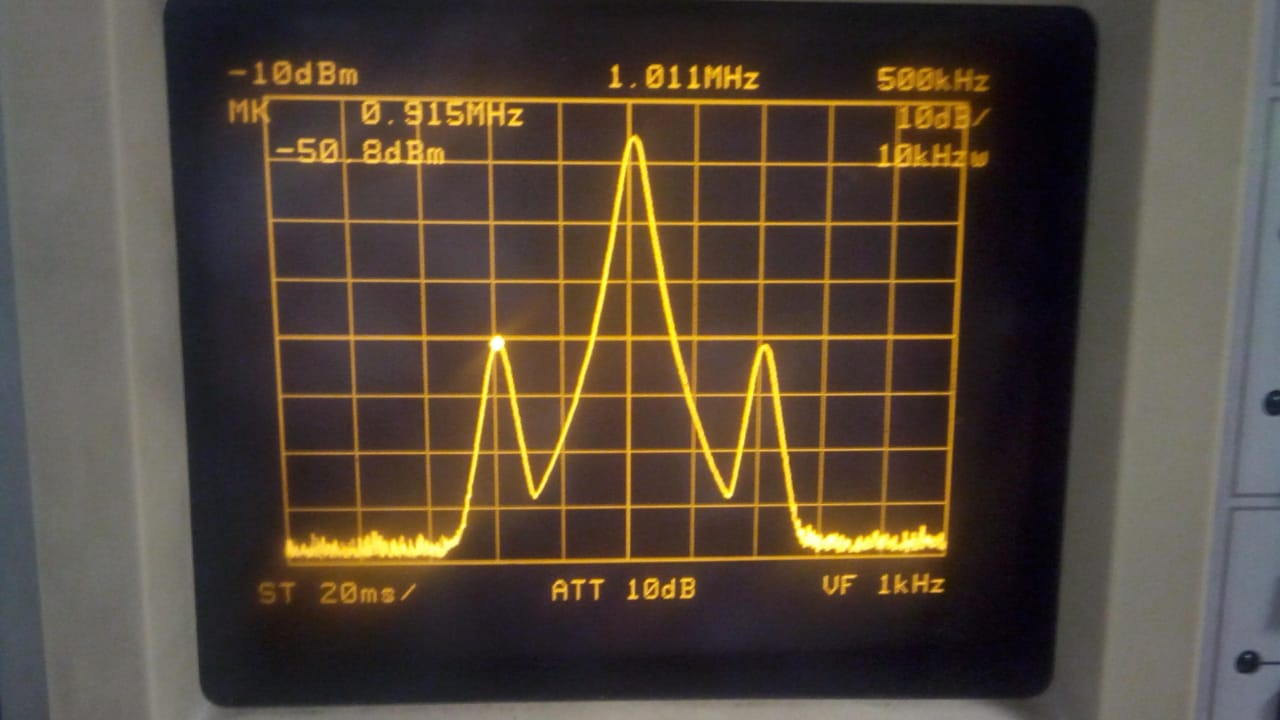
\includegraphics[width=\textwidth]{/ImagenesEjercicio3y4/AM05_4.jpeg}
    \caption{Espectro de la señal AM con m=0,5}
    \label{fig:am02}
  \end{minipage}
\end{figure}

Puede observarse que la diferencia entre el pico central y los escoltas es de aproximadamente $100 kHz$, lo cual corresponde a lo esperado, ya que la frecuencia de la moduladora era de $100 kHz$. Además, puede apreciarse que el pico central está a una frecuencia de $1,011 MHz$, muy cercana a la frecuencia que se configuró para la señal portadora de $1 Mhz$.

\subsection{Señal senoidal AM m=1}

En este caso se observa que mientras la amplitud del pico central se mantuvo igual, la de ambas escoltas aumentó. La diferencia de frecuencias continúa siendo de alrededor de $100 KHz$. Se observa que el pico central se encontró en $0,92 MHz$. Se realizó una simulación del espectro que se observa en la figura (\ref{fig:simsin}). En las Figuras (\ref{fig:am1}) y (\ref{fig:am2}) se puede observar el espectro medido en el analizador.

\begin{figure}[H]
	\centering
	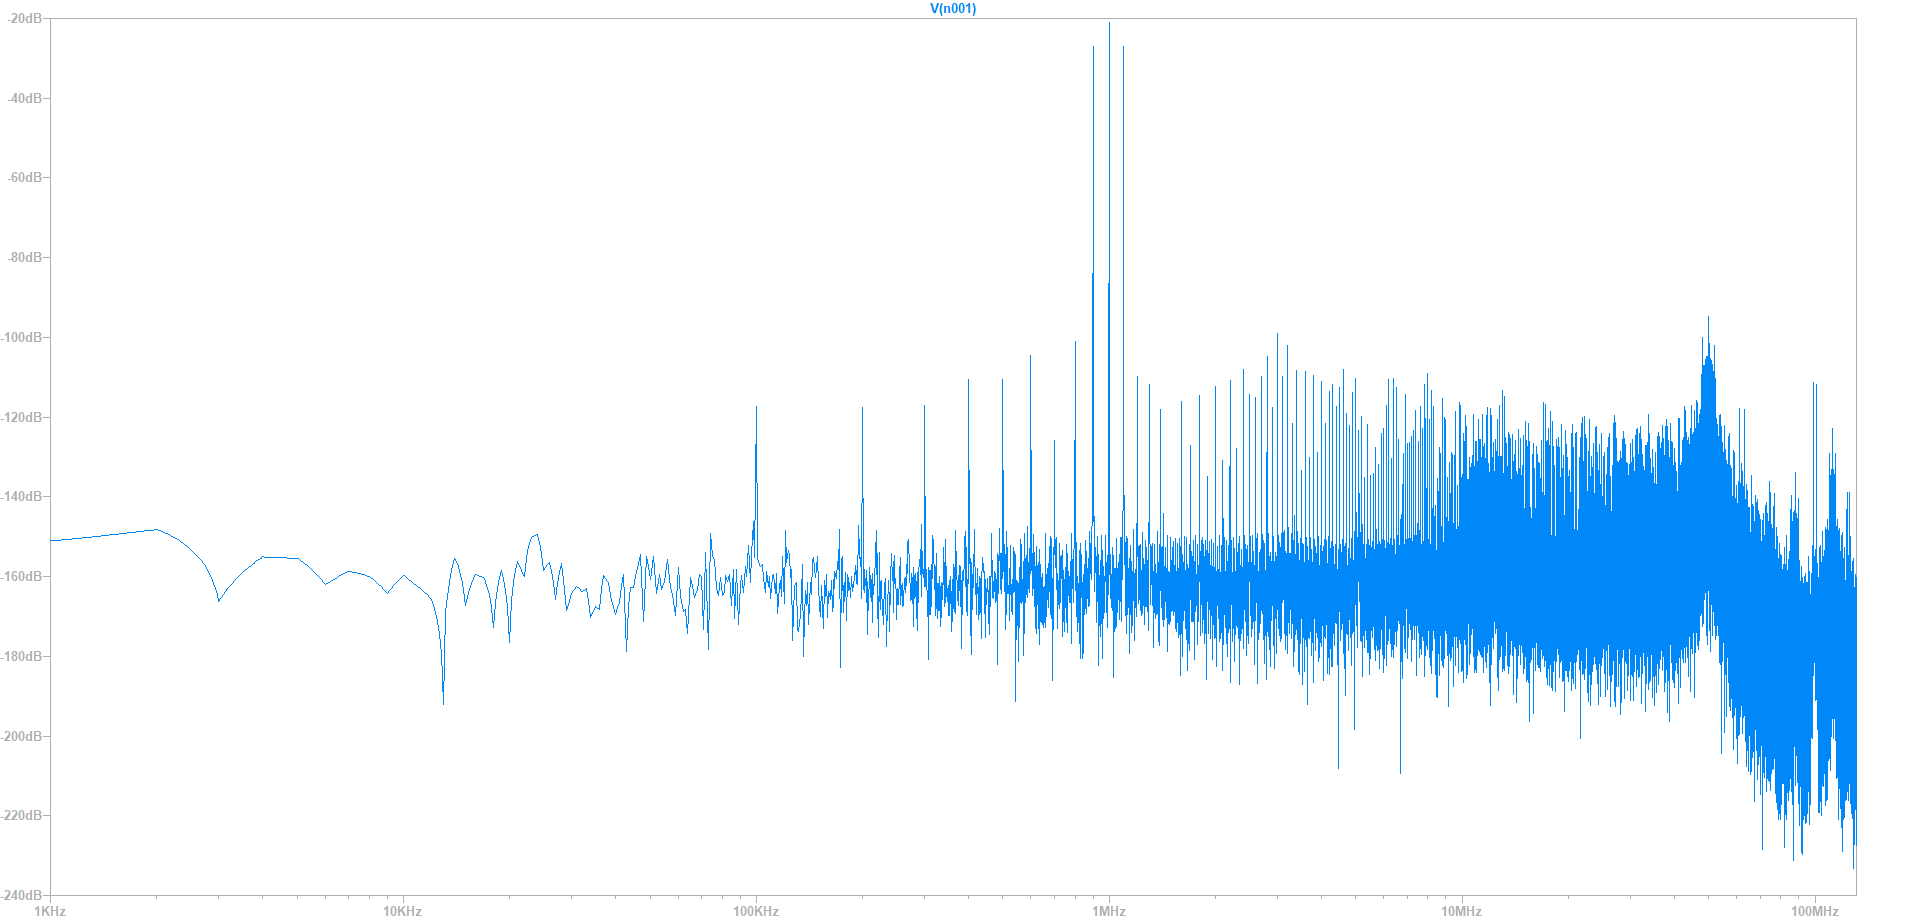
\includegraphics[width=0.9\textwidth]{/ImagenesEjercicio3y4/FFT-AM-Sin-m1.png}
\caption{Espectro simulado de la señal AM con m=1}
	\label{fig:simsin}
\end{figure}

\begin{figure}[H]
  \centering
  \begin{minipage}[b]{0.6\textwidth}
    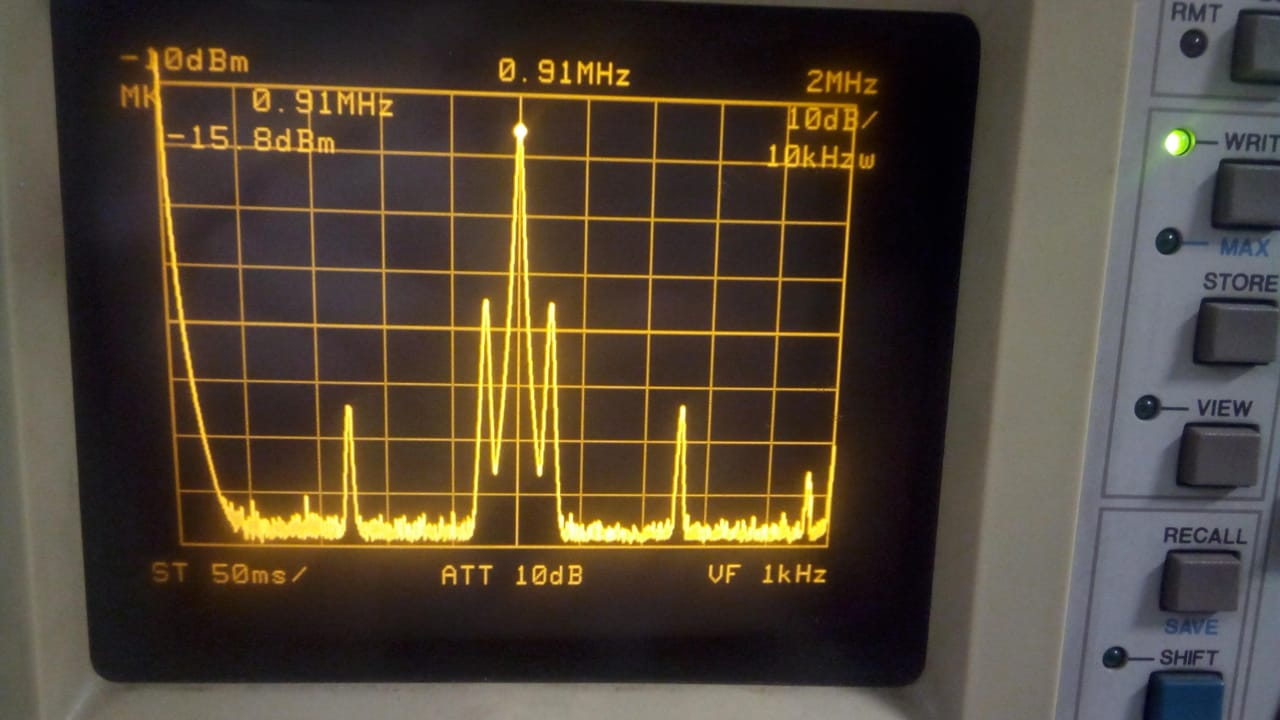
\includegraphics[width=\textwidth]{/ImagenesEjercicio3y4/AM1_2.jpeg}
    \caption{Espectro de la señal AM con m=1}
    \label{fig:am1}
  \end{minipage}
  \hfill
  \begin{minipage}[b]{0.6\textwidth}
    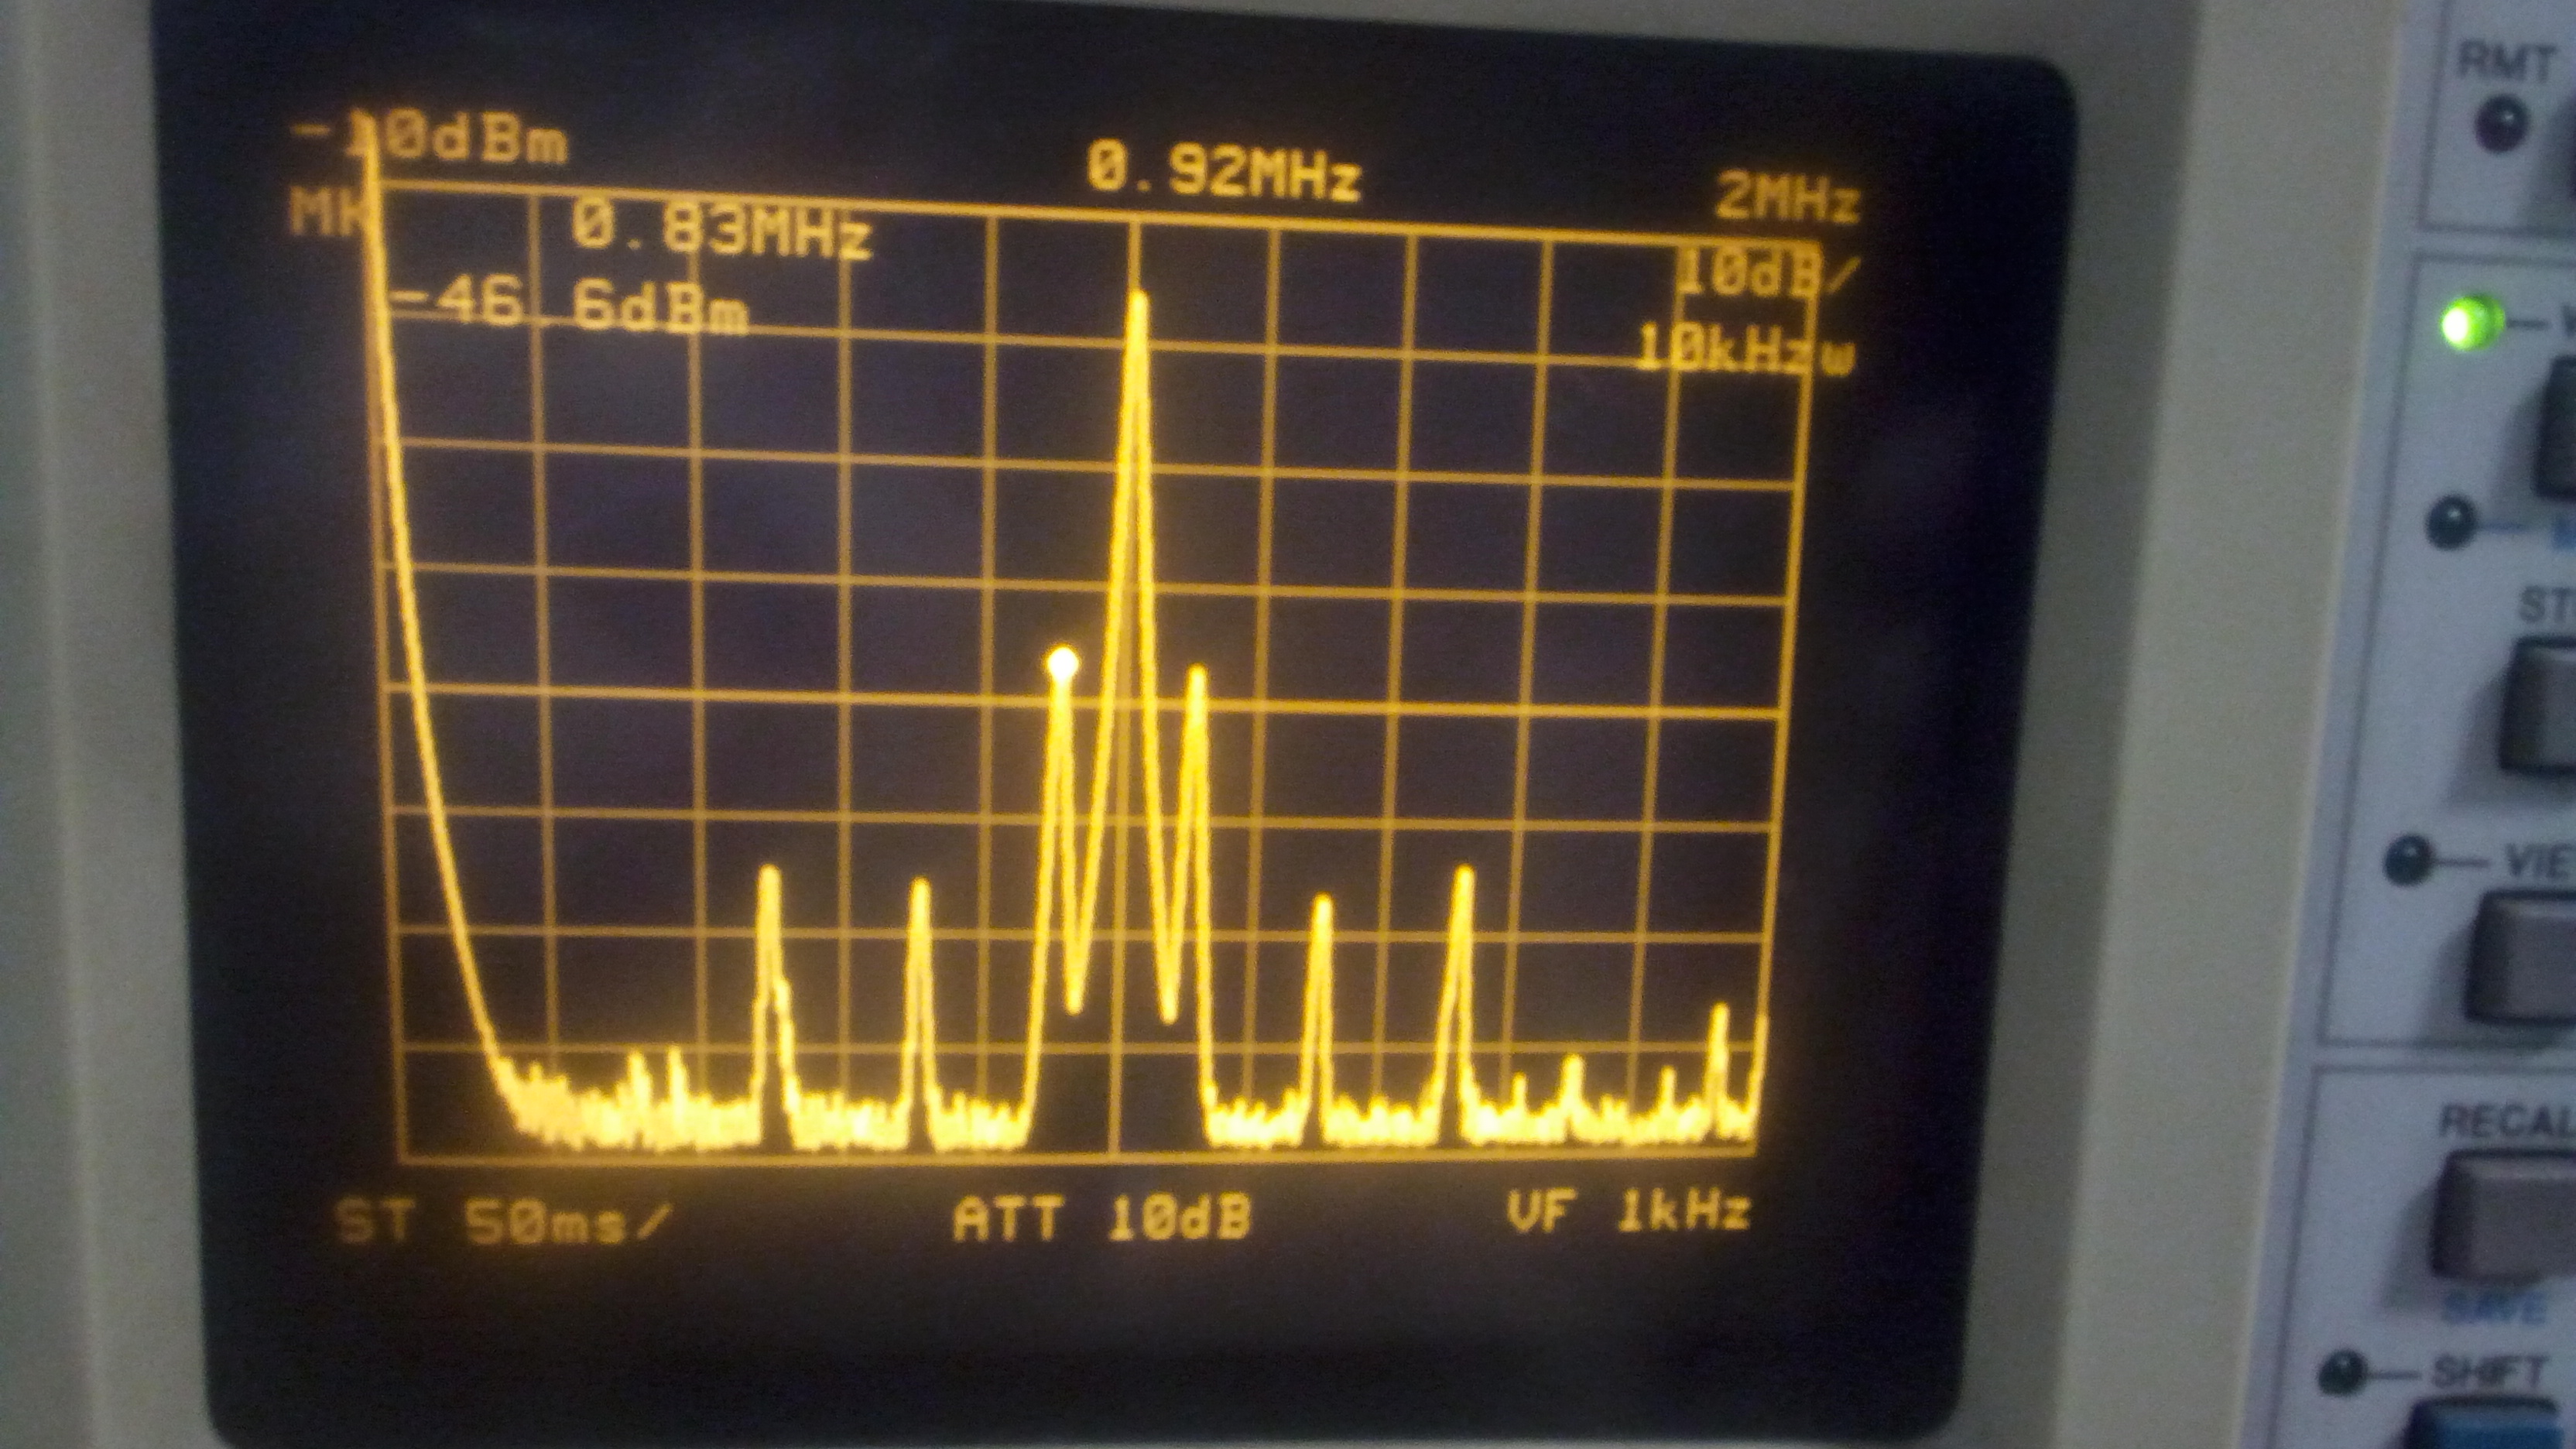
\includegraphics[width=\textwidth]{/ImagenesEjercicio3y4/AM12.jpg}
    \caption{Espectro de la señal AM con m=1}
    \label{fig:am2}
  \end{minipage}
\end{figure}

\subsection{Señal triangular AM con m=1}
Se analizó una señal triangular con $m=1$. En este caso se observó la aparición de más armónicos que antes. En la figura (\ref{fig:simtri}) se observa una simulación del espectro a medir. En la figura (\ref{fig:trign}) se puede observar el espectro medido.

\begin{figure}[H]
	\centering
	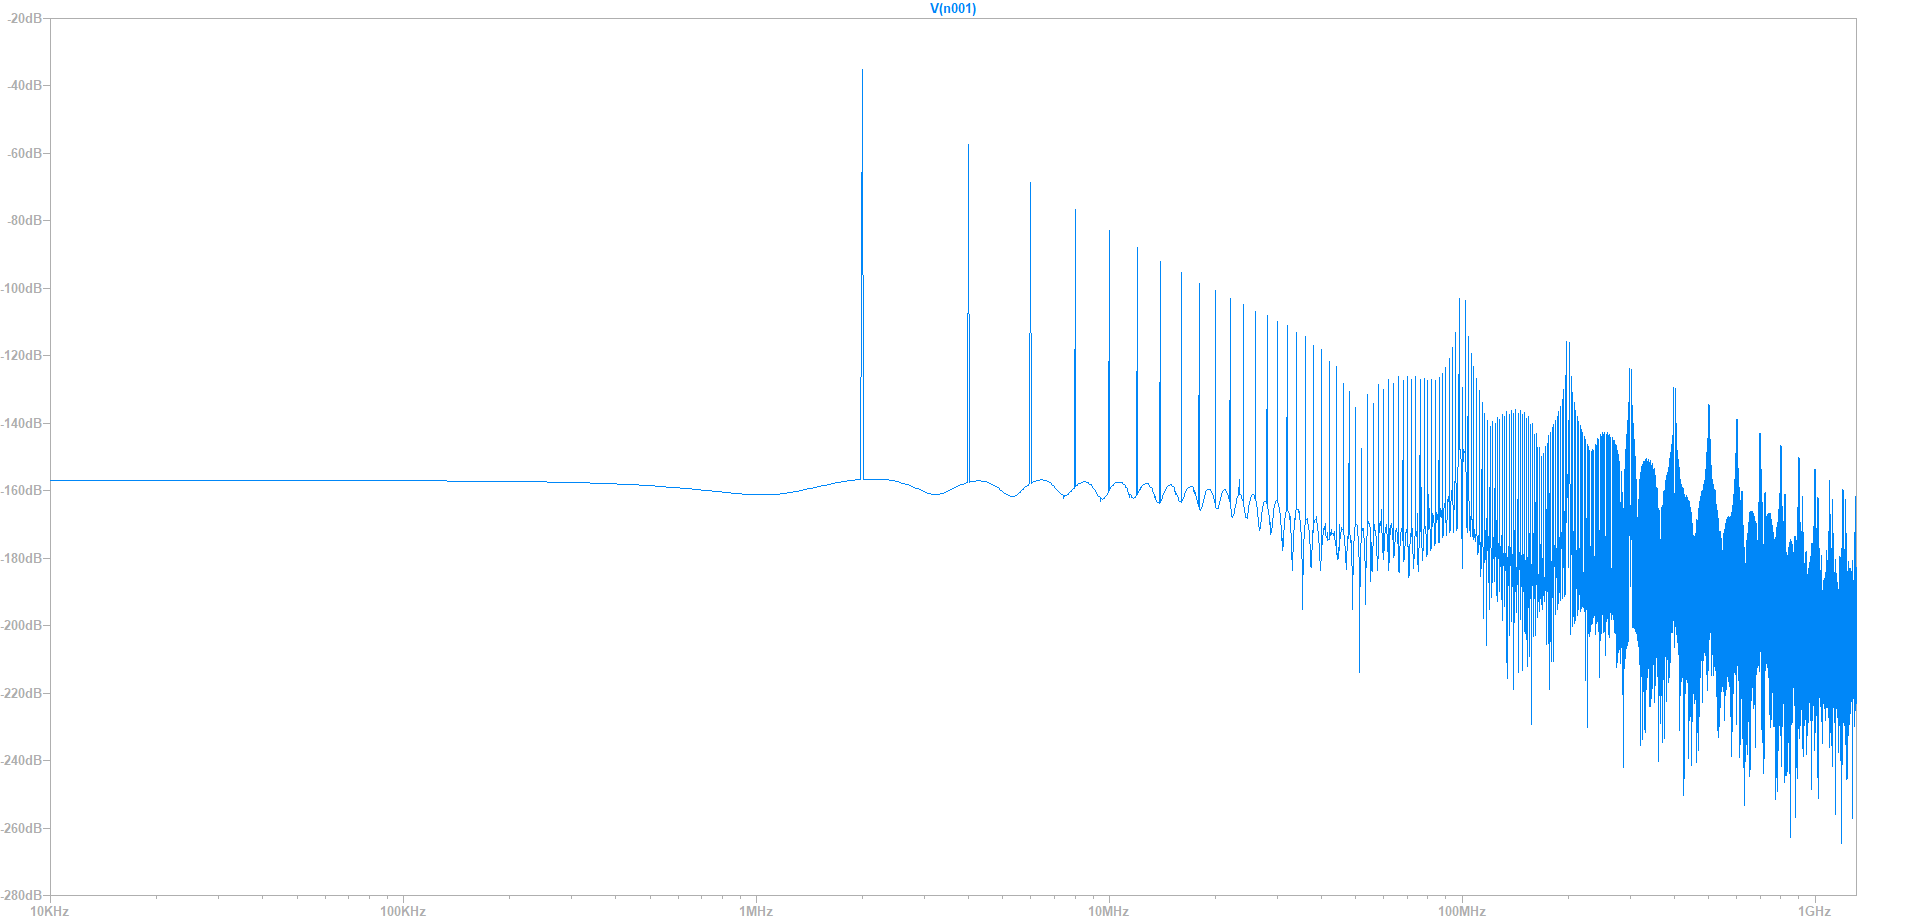
\includegraphics[width=0.9\textwidth]{/ImagenesEjercicio3y4/FFT-AM-Triang.png}
\caption{Espectro simulado de la señal triangular AM}
	\label{fig:simtri}
\end{figure}


\begin{figure}[H]
	\centering
	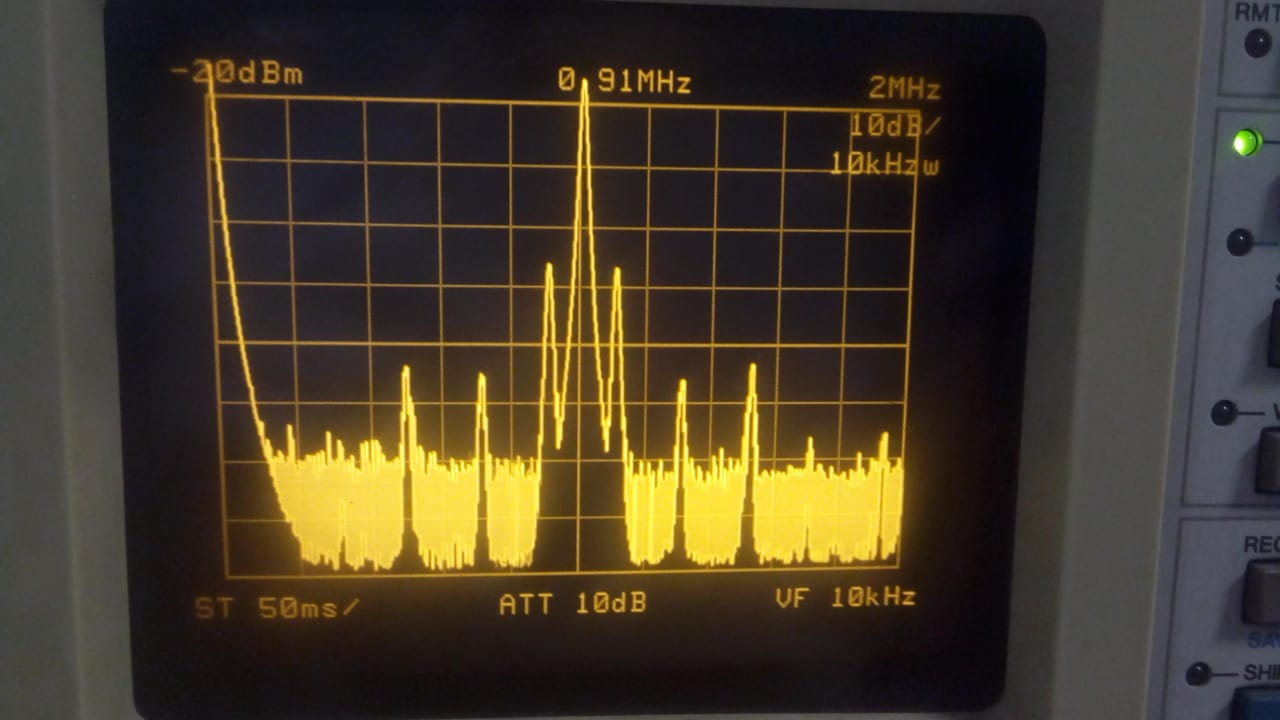
\includegraphics[width=0.9\textwidth]{/ImagenesEjercicio3y4/AMT_4.jpeg}
\caption{Espectro de señal triangular AM con m=1}
	\label{fig:trign}
\end{figure}

\subsection{Señal senoidal AM con f=1 MHz, m=1 }

Se analizó nuevamente una señal senoidal AM con m=1 pero ahora la frecuencia de la moduladora se hizo coincidir con la de la portadora. En este caso, la separación entre la frecuencia central y la escolta debería corresponder a $f_m+f_p=2f_p$ siendo $f_m$ la frecuencia de la moduladora y $f_p$ la frecuencia de la portadora. En la figura (\ref{fig:simsin1}) puede observarse el espectro simulado. En la Figura (\ref{fig:amff}) se observa el espectro medido.

\begin{figure}[H]
	\centering
	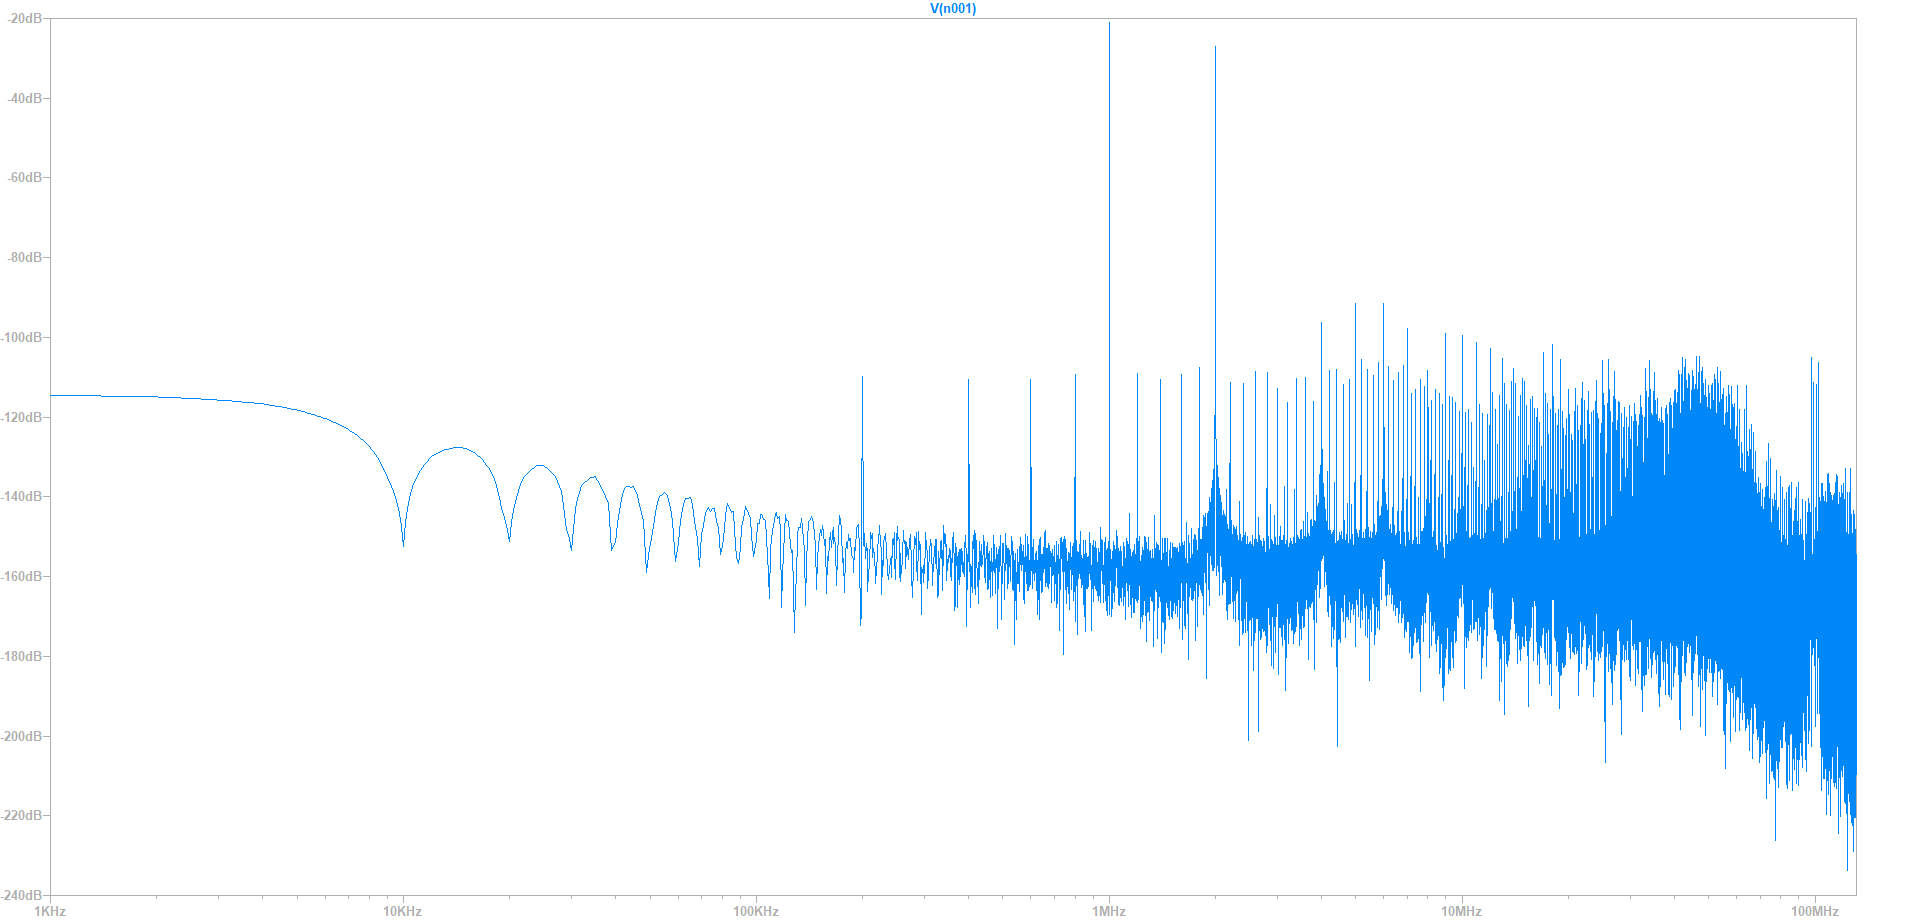
\includegraphics[width=0.9\textwidth]{/ImagenesEjercicio3y4/FFT-AM-Sin-m1-1MHZ.png}
\caption{Espectro simulado de la señal senoidal con m=1 y f=fp}
	\label{fig:simsin1}
\end{figure}

\begin{figure}[H]
	\centering
	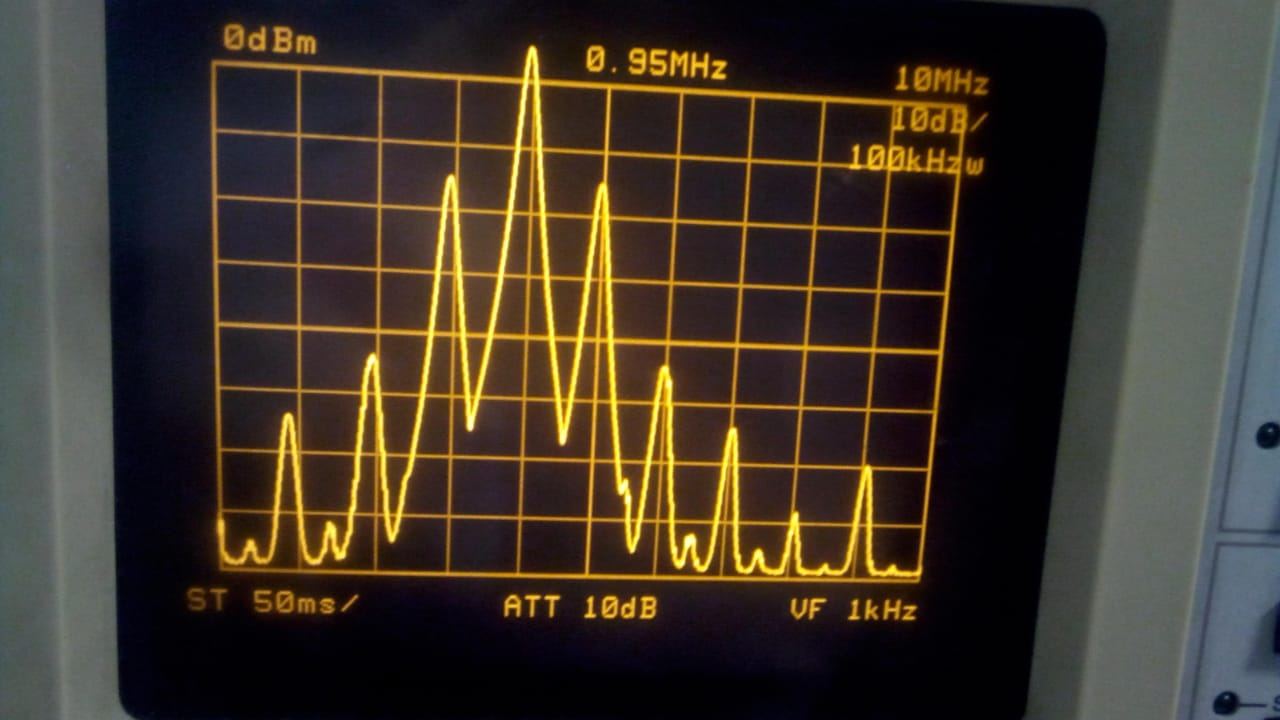
\includegraphics[width=0.9\textwidth]{/ImagenesEjercicio3y4/AMf_1.jpeg}
\caption{Espectro de senoidal AM con f=fp y m=1}
	\label{fig:amff}
\end{figure}

\section{Análisis de señales FM}

En esta parte se estudiaron señales moduladas en FM. Al igual que en el estudio de la modulación en AM se utilizó una señal moduladora de frecuencia $100 kHz$ y una portadora de frecuencia $1 MHz$ y amplitud de $250 mV_{pp}$.

\subsection{Señal senoidal FM con m=0,5}
Nuevamente se modificó la amplitud de la moduladora en la mitad de la amplitud de la portadora, para lograr lo que en AM correspondería a un $m=0,5$. En las Figuras (\ref{fig:fm05}) y (\ref{fig:fm055}) se presenta el espectro medido en el analizador. Puede observarse un aumento en la cantidad de armónicos, al igual que en la potencia de cada uno; la diferencia entre la frecuencia central y las primeras "escoltas" sigue siendo de $100 kHz$.

\begin{figure}[H]
  \centering
  \begin{minipage}[b]{0.6\textwidth}
    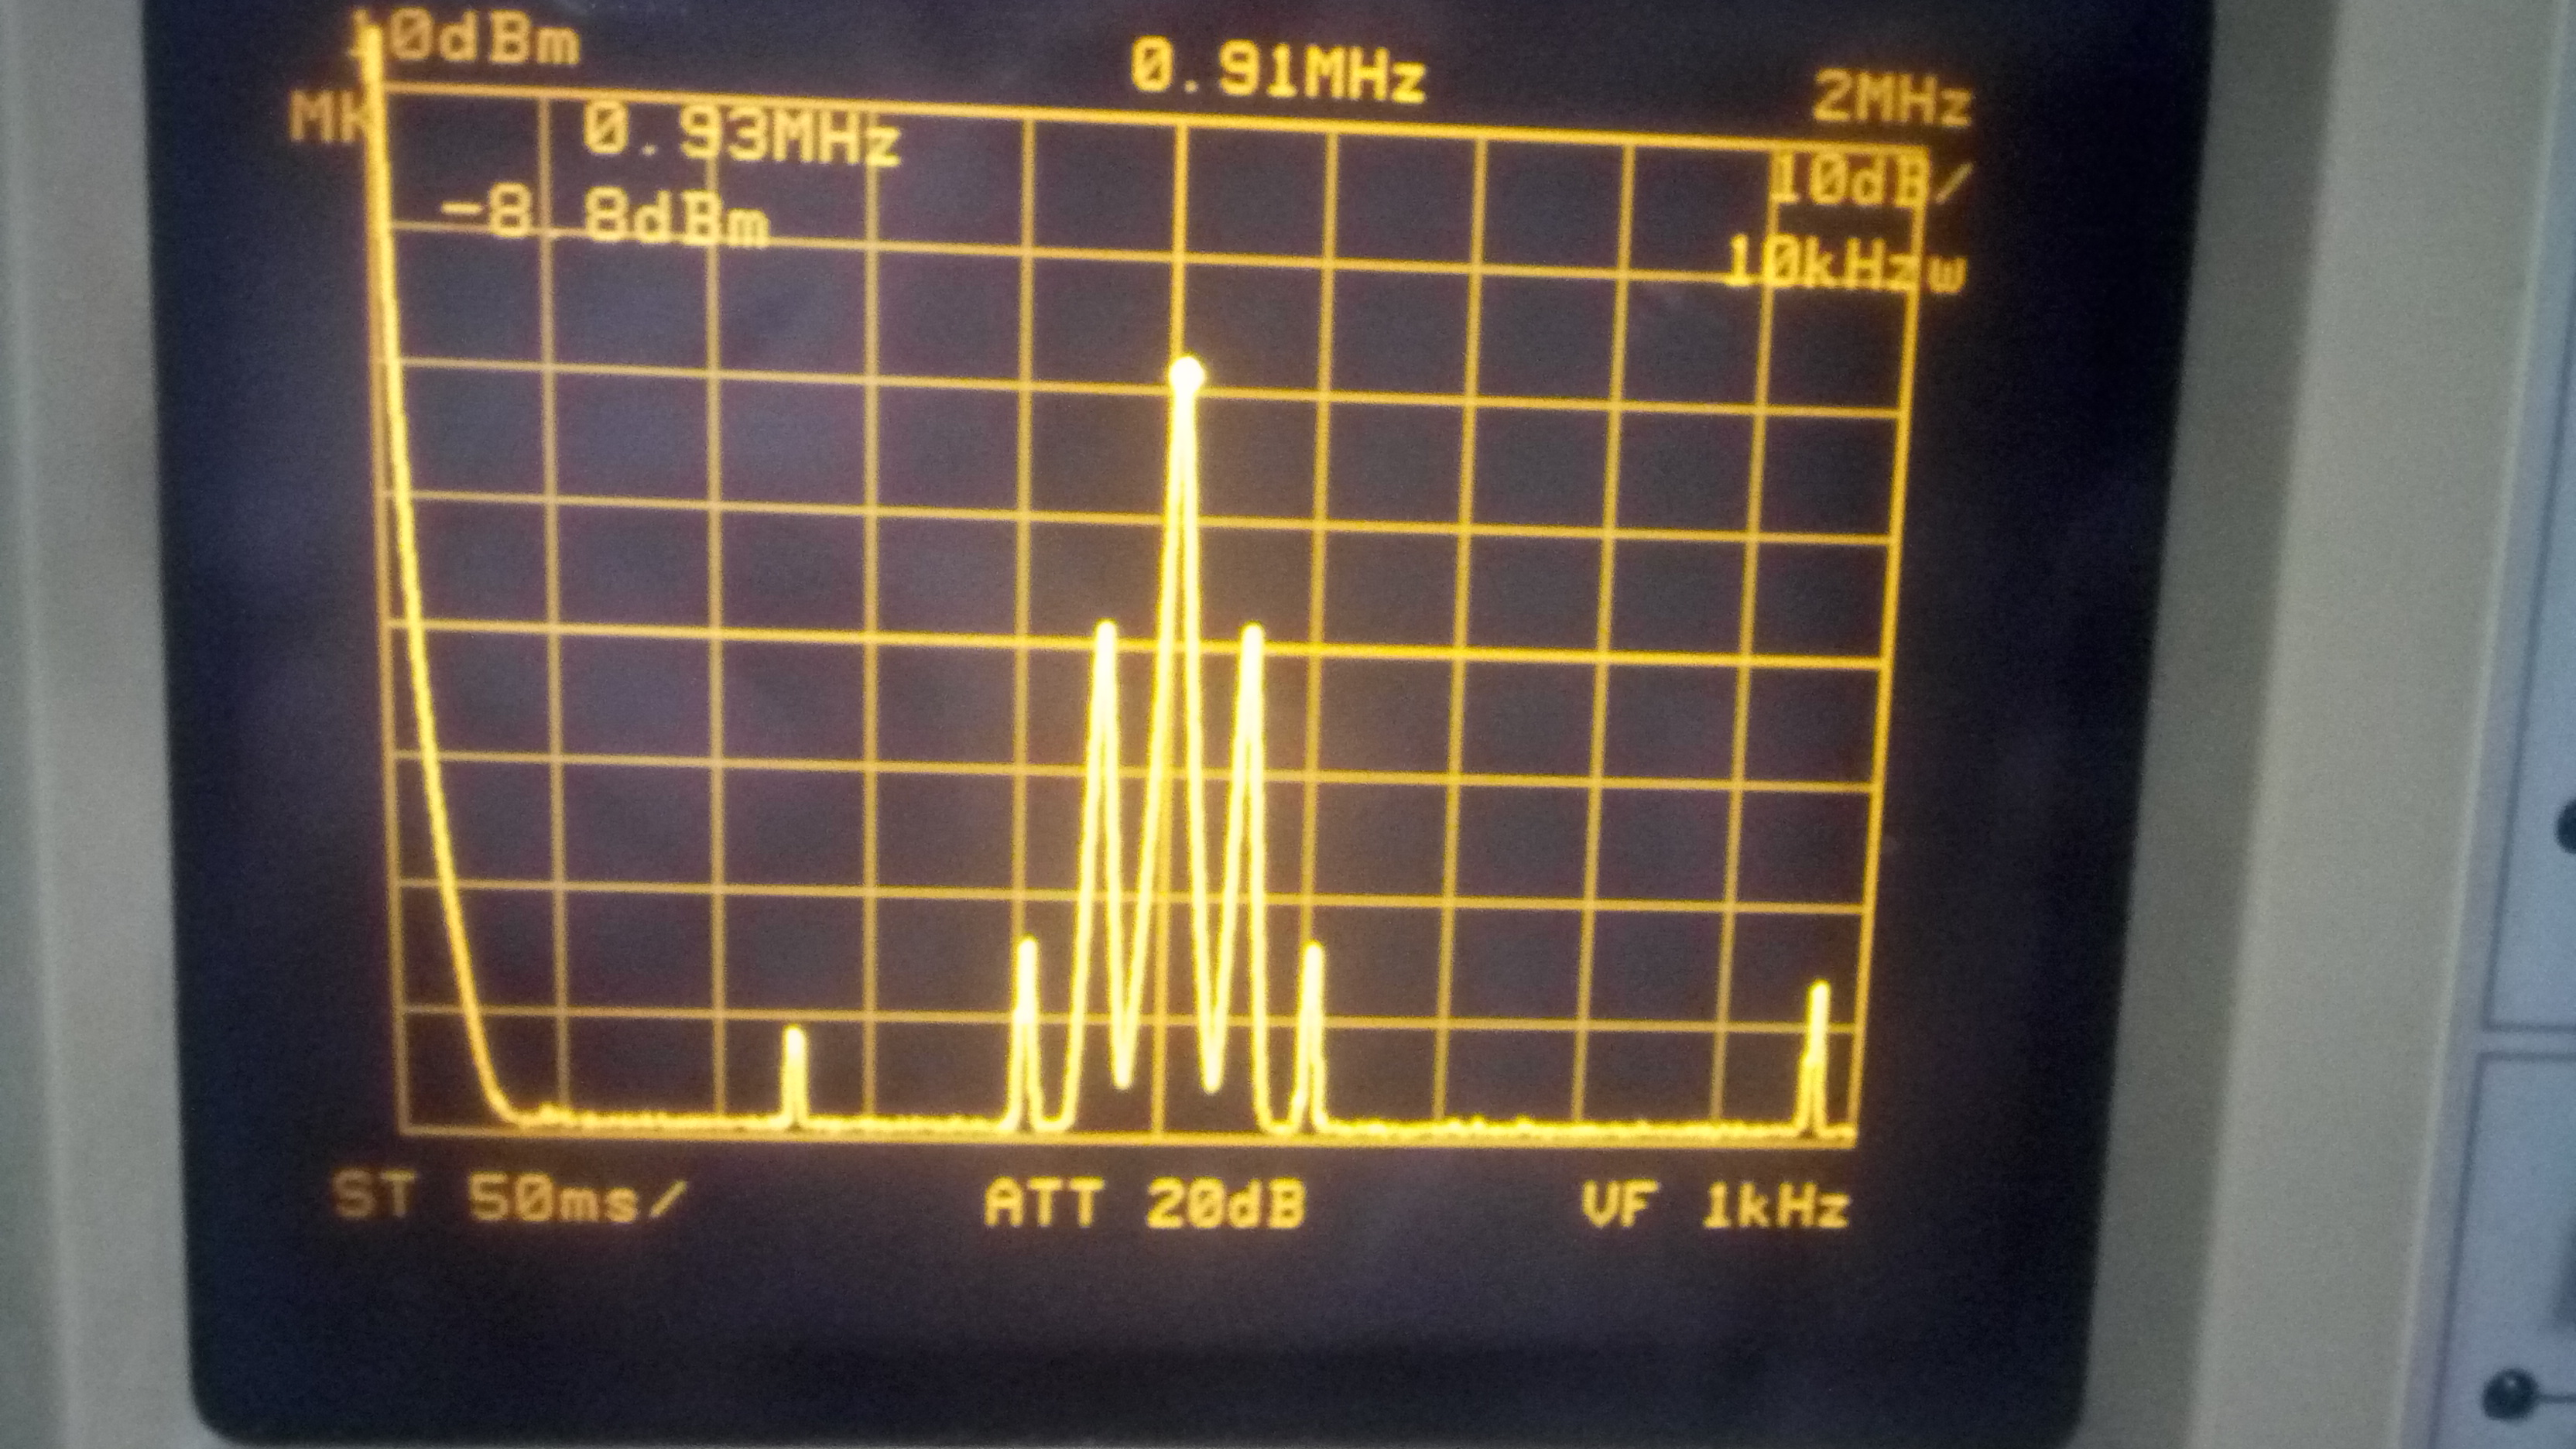
\includegraphics[width=\textwidth]{/ImagenesEjercicio3y4/FM05.jpg}
    \caption{Señal senoidal FM con m=0,5}
    \label{fig:fm05}
  \end{minipage}
  \hfill
  \begin{minipage}[b]{0.6\textwidth}
    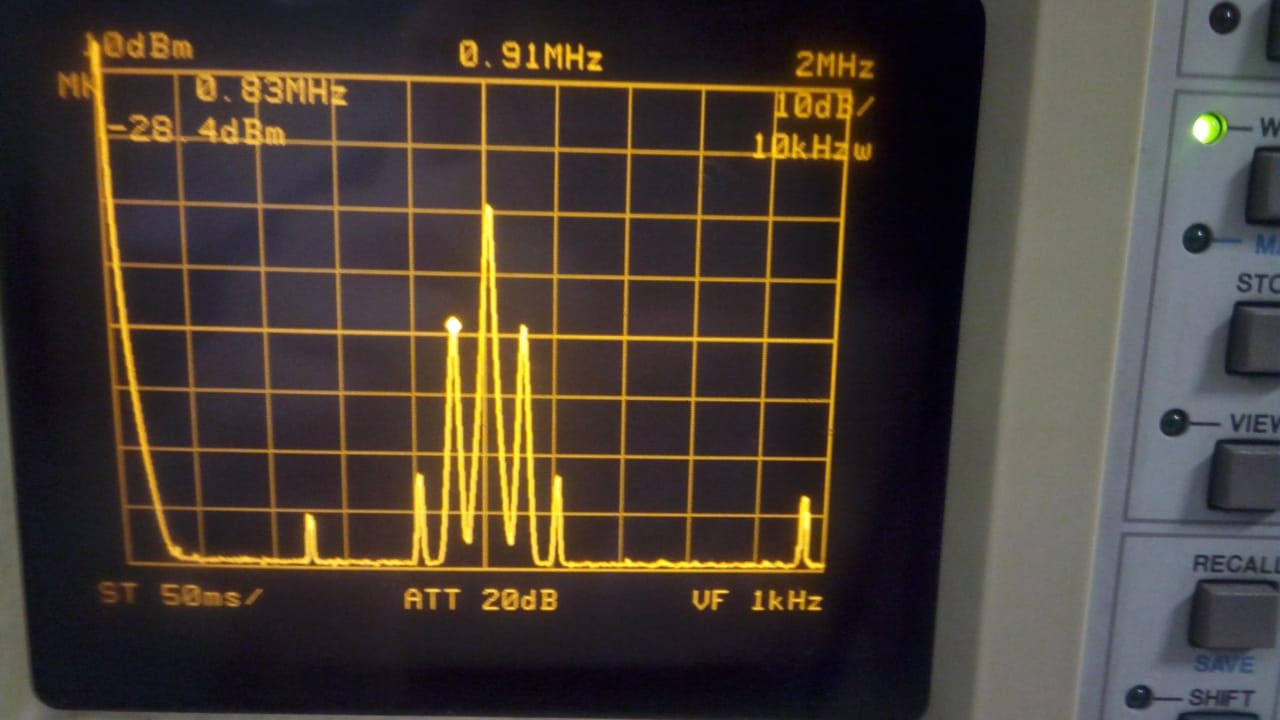
\includegraphics[width=\textwidth]{/ImagenesEjercicio3y4/FM0,5_2.jpeg}
    \caption{Señal senoidal FM con m=0,5}
    \label{fig:fm055}
  \end{minipage}
\end{figure}

\subsection{Señal senoidal FM con m=1}
Se configuró la amplitud de la moduladora en $250 mV_{pp}$ para que coincidiera con la amplitud de la portadora. Una vez más se observó la aparición de nuevos armónicos y el aumento de la potencia de cada uno comparado con el caso AM. La diferencia entre la frecuencia central y las escoltas se mantiene en $100 kHz$. Las Figuras (\ref{fig:fm1}) y (\ref{fig:fm1_5}) presentan lo observado en el analizador.

\begin{figure}[H]
  \centering
  \begin{minipage}[b]{0.6\textwidth}
    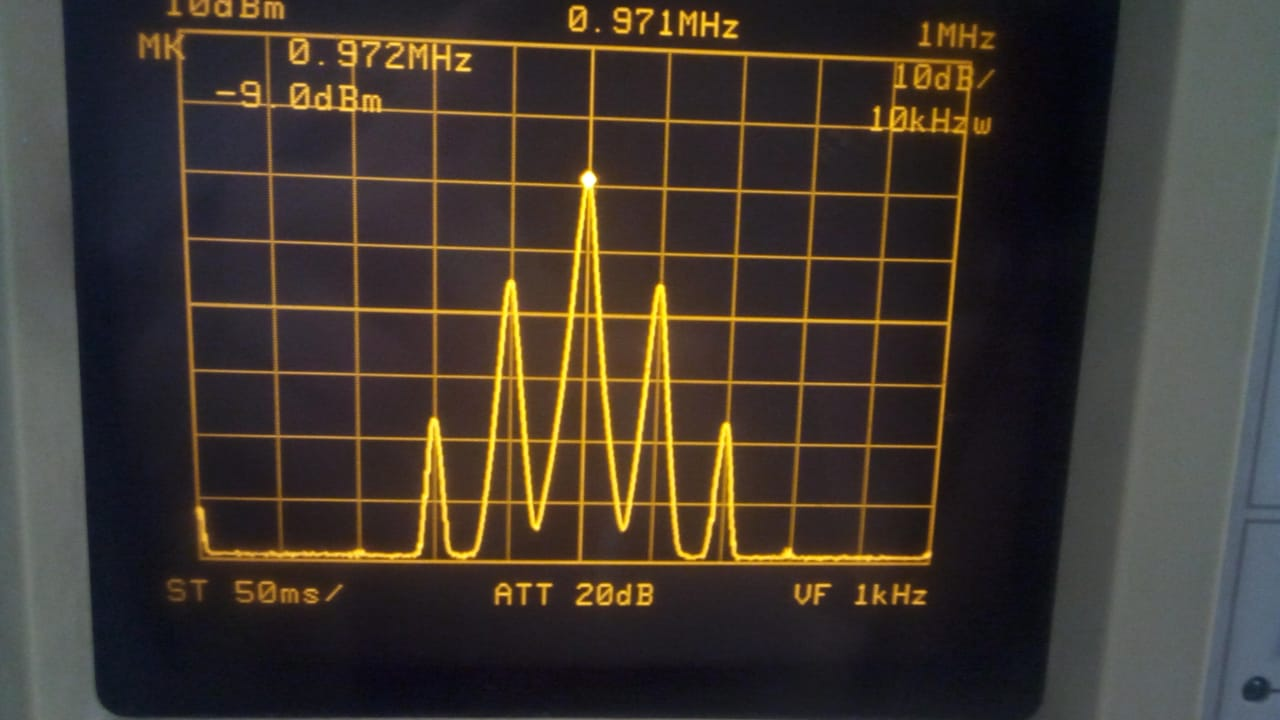
\includegraphics[width=\textwidth]{/ImagenesEjercicio3y4/FM1_3.jpeg}
    \caption{Señal senoidal FM con m=1}
    \label{fig:fm1}
  \end{minipage}
  \hfill
  \begin{minipage}[b]{0.6\textwidth}
    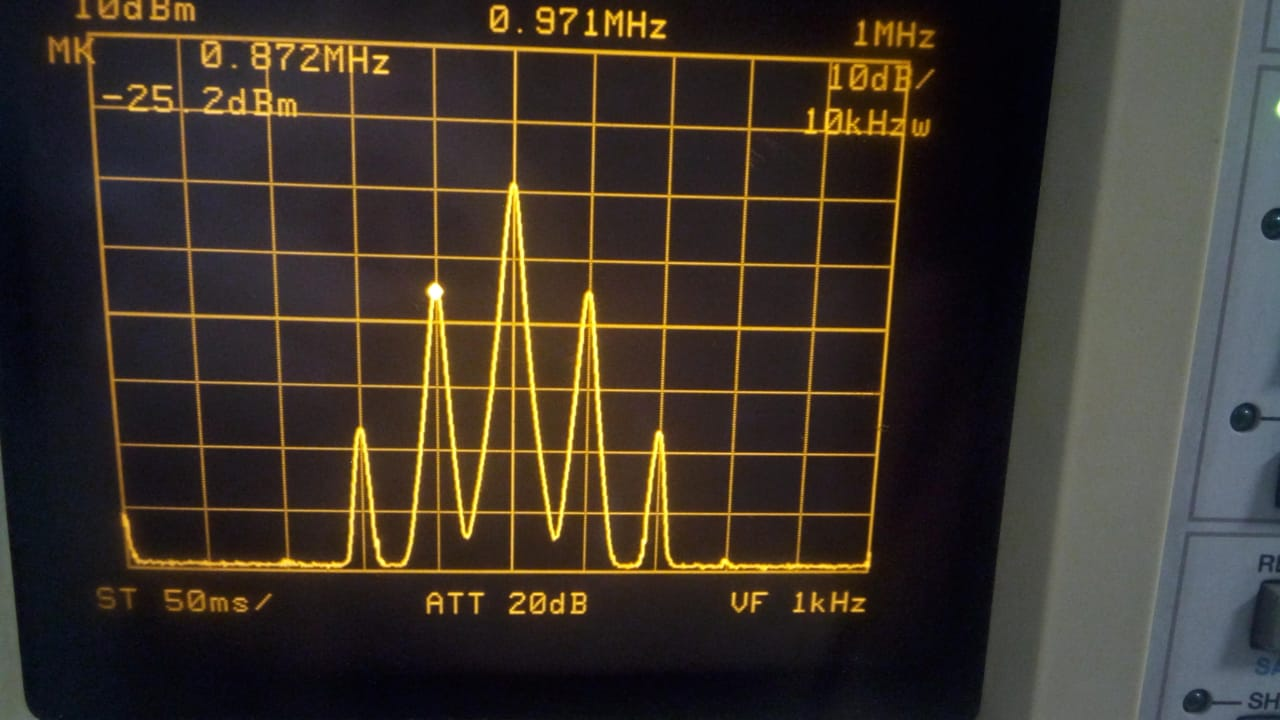
\includegraphics[width=\textwidth]{/ImagenesEjercicio3y4/FM1_2.jpeg}
    \caption{Señal senoidal FM con m=1}
    \label{fig:fm1_5}
  \end{minipage}
\end{figure}

\subsection{Señal triangular FM}
Nuevamente se analizó una señal triangular, pero en este caso modulada en FM. Al igual que en los dos casos anteriores se aprecia la aparición de nuevos armónicos. La Figura (\ref{fig:fmt1}) muestra lo observado en el analizador.

\begin{figure}[H]
	\centering
	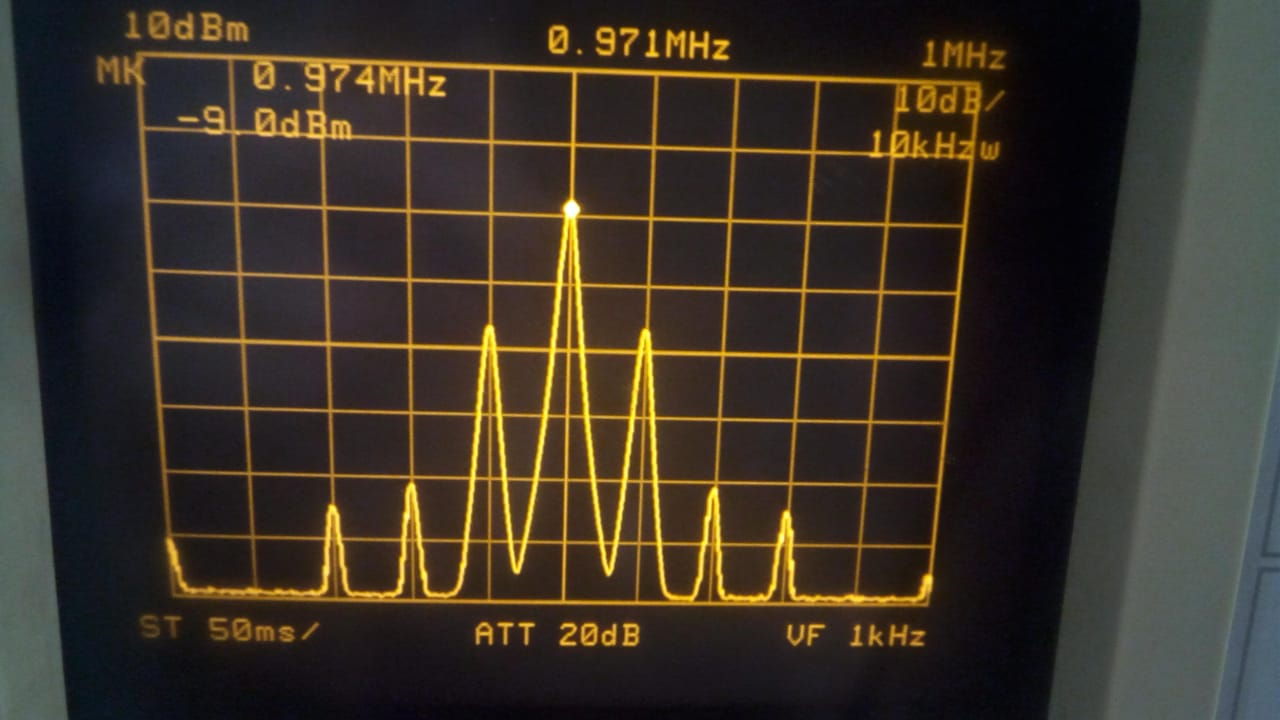
\includegraphics[width=0.9\textwidth]{/ImagenesEjercicio3y4/FMT_5.jpeg}
\caption{Señal triangular modulación FM}
	\label{fig:fmt1}
\end{figure}\textbf{}

\subsection{Señal senoidal FM con fm=1 MHz}

Se configuró la amplitud de la señal moduladora al mismo valor que la de la señal portadora. En la figura \ref{fig:fmf} se muestra lo observado en el analizador.

\begin{figure}[H]
	\centering
	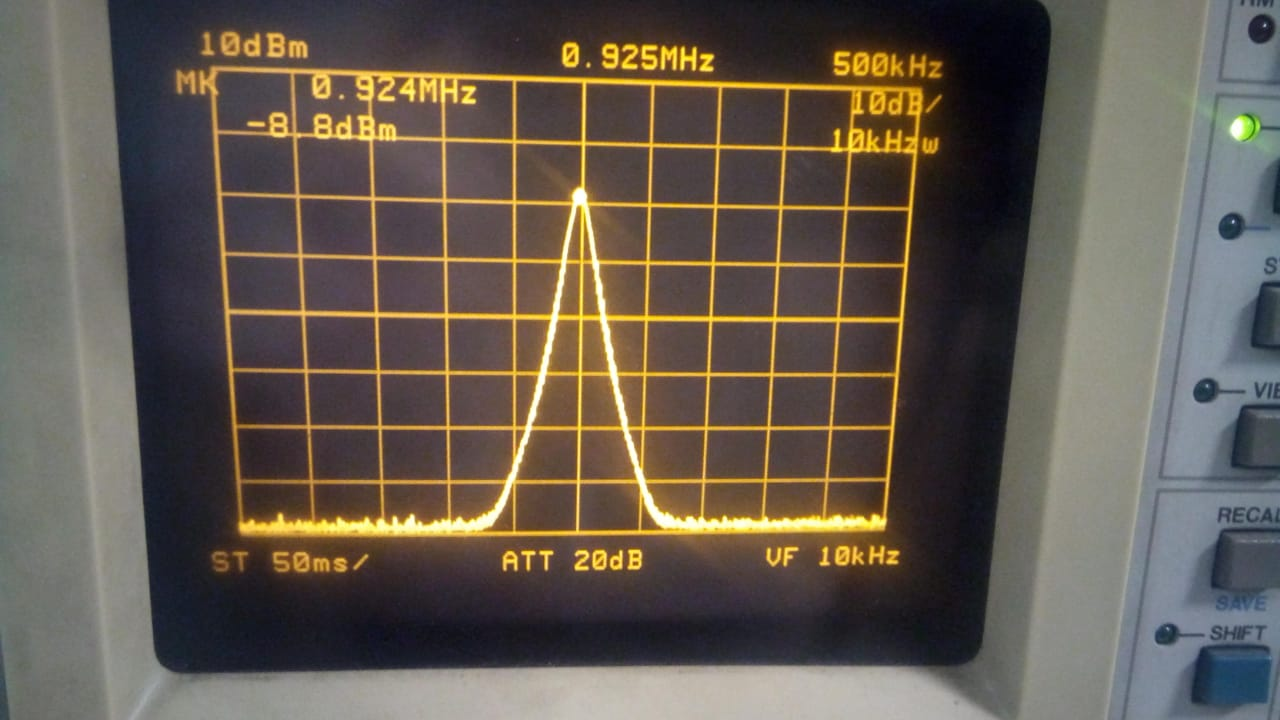
\includegraphics[width=0.9\textwidth]{/ImagenesEjercicio3y4/FMf_1.jpeg}
\caption{Señal senoidal FM con f=fp}
	\label{fig:fmf}
\end{figure}
